% Sandia National Laboratories is a multimission laboratory managed and
% operated by National Technology & Engineering Solutions of Sandia, LLC, a
% wholly owned subsidiary of Honeywell International Inc., for the U.S.
% Department of Energy’s National Nuclear Security Administration under
% contract DE-NA0003525.

% Copyright 2002-2020 National Technology & Engineering Solutions of Sandia,
% LLC (NTESS).


\begin{Device}

\symbol
{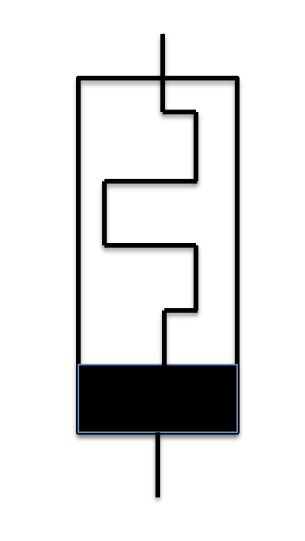
\includegraphics[scale=.2, angle=90]{MemristorSymbol}}

\device
ymemristor <name> <(+) node> <(-) node> <model>

\model
\begin{alltt}
.MODEL <model name> MEMRISTOR level=2 [model parameters]
\end{alltt}

\examples
\begin{alltt}

ymemristor mr1 n1 n2 mrm2

.model mrm2 memristor level=2 ron=50 roff=1000 
+ koff=1.46e-18 kon=-4.68e-22 
+ alphaoff=10 alphaon=10 wc=1.0e-12 
+ ioff=115e-6 ion=-8.9e-6 xscaling=1.0e9 wt=4


ymemristor mr2 n1 n2 mrm3 xo=0.11 

.MODEL mrm3 memristor level=3 a1=0.17 a2=0.17 b=0.05 vp=0.16 vn=0.15 
+ ap=4000 an=4000 xp=0.3 xn=0.5 alphap=1 alphan=5 eta=1 


ymemristor mr3 n1 n2 mrm4 

.model mrm4 memristor level=4 
+ fxpdata=fxp_table.csv
+ fxmdata=fxm_table.csv
+ I1=85.37e-6 I2=90.16e-6 V1=0.265 V2=0.265 G0=130.72e-6
+ VP=0.7 VN=1.0 d1=9.87 d2=-4.82
+ C1=1000 C2=1000

\end{alltt}

\parameters

\begin{Parameters}
\param{\vbox{\hbox{(+) node\hfil}\hbox{(-) node}}}

Polarity definition for a positive voltage across the memristor. The
first node is defined as positive. Therefore, the voltage across the
component is the first node voltage minus the second node voltage.


\end{Parameters}

\comments
The {\tt level=2} memristor device is an implementation of the TEAM formulation described 
in~\cite{KvatinskyFriedman2012} and~\cite{KvatinskyFriedman2013}.
The {\tt level=3}  memristor device is an implementation of the Yakopcic formulation described 
in~\cite{ChrisYakopcic2013}. The {\tt level=4} memristor device is an implementation of the 
Piecewise Empirical Model described in~\cite{Niroula2017}.

Positive current flows from
the \texttt{(+)} node through the device to the \texttt{(-)}
node. The power through the device is calculated 
with $I \cdot \Delta V$ where the voltage drop is calculated as $(V_+ - V_-)$ 
and positive current flows from $V_+$ to $V_-$.  
\end{Device}

\paragraph{Device Equations for TEAM Formulation}
The current voltage relationship for the TEAM formulation can be linear or nonlinear and this is selectable with 
the instance parameter {\tt IVRELATION}.  The default is the linear relationship which is:
\begin{equation}
v(t) = \left[ R_{ON} + \frac{R_{OFF} - R_{ON}}{x_{OFF} - x_{ON}} \left( x - x_{ON} \right) \right] i(t)
\end{equation}
The non-linear relationship is:
\begin{equation}
v(t) = R_{ON} e^{\lambda(x - x_{ON})/(x_{OFF}-x_{ON})}  i(t)
\end{equation}
where $\lambda$ is defined as:
\begin{equation}
\frac{R_{OFF}}{R_{ON}} = e^{\lambda}
\end{equation}
In the above equations $x$ represents a doped layer whose growth determines the overall
resistance of the device.  The equation governing the value of $x$ is:
\begin{equation}
\frac{dx}{dt} = \left\{  
  \begin{array}{ll}
    k_{OFF} \left(\frac{i}{i_{OFF}} - 1 \right)^{\alpha_{OFF}} f_{OFF}(x) & 0 < i_{OFF} < i \\
    0       & i_{ON} < i < i_{OFF} \\
    k_{ON} \left(\frac{i}{i_{on}} - 1 \right)^{\alpha_{on}} f_{ON}(x) & i < i_{ON} < 0 \\
  \end{array}
  \right.
\end{equation}

The functions $f_{ON}(x)$ and $f_{OFF}(x)$ are window functions designed to keep $x$ within
the defined limits of $x_{ON}$ and $x_{OFF}$.  Four different types of window functions 
are available and this is selectable with the model parameter {\tt WT}. Note that the 
TEAM memristor device is formulated to work best with the TEAM, Kvatinsky, window 
function {\tt WT=4 }.  Other window functions should be used with caution.

\paragraph{Device Equations for Yakopcic Formulation}
The current voltage relationship for the Yakopcic memristor device is:~\cite{ChrisYakopcic2013}
\begin{equation}
I(t) = \left\{  
  \begin{array}{ll}
    a_1 x(t) \sinh(b V(t)) & V(t) \ge 0 \\
    a_2 x(t) \sinh(b V(t)) & V(t) < 0 \\
  \end{array}
  \right.
\end{equation}

\begin{equation}
g(V(t)) = \left\{  
  \begin{array}{ll}
    A_p\left( \exp^{V(t)} - \exp^{V_p}\right) & V(t) > V_p \\
    -A_n \left( \exp^{-V(t)} - \exp^{V_n}\right) & V(t) < -V_n \\
    0       & -V_n \le V(t) \le V_p \\
  \end{array}
  \right.
\end{equation}

The internal state variable, $x$, is governed by the equation:

\begin{equation}
\frac{dx}{dt} = n g(V(t)) f(x(t))
\end{equation}

where $f(x)$ is defined by:

\begin{equation}
f(x) = \left\{  
  \begin{array}{ll}
   \exp^{-\alpha_p (x-x_p)} w_p(x,x_p) & x \ge x_p \\
   1 & x \le x_p \\
  \end{array}
  \right.
\end{equation}
\begin{equation}
f(x) = \left\{  
  \begin{array}{ll}
   \exp^{\alpha_n (x+x_n-1} w_n(x,x_n) & x \le 1-x_n \\
   1 & x > 1 - x_n \\
  \end{array}
  \right.
\end{equation}
\begin{equation}
w_p(x,x_p) = \frac{x_p -x}{1 - x_p} + 1
\end{equation}
\begin{equation}
w_n(x,x_n) = \frac{x}{1-x_n}
\end{equation}

Note, the quantities, $x_p$, $x_n$, $\alpha_p$, $\alpha_n$, $A_p$, $A_n$, $a_1$, $a_2$ and$b$ are model
parameters that can be specified in the device's model block.


\paragraph{Device Equations for the PEM Formulation}
The PEM memristor device is similar to the TEAM and Yakopcic formulations in that an 
internal state variable, $x$, is used to capture the device's response to its history.

The I-V relationship is
\begin{equation}
I = x \: h(V)
\end{equation}

and $h(V)$ is defined by:
\begin{equation}
 h(V) = I_1 * exp(V/V_1) - I_2 * exp(-V/V_2) + G_0 V - (I_1-I_2)
\end{equation}
where $I_1$, $I_2$, $V_1$, $V_2$ and $G_0$ are model parameters.

The internal variable, $x$, is defined by:
\begin{equation}
  \frac{dx}{dt} = G(V) f(x)
\end{equation}
with
\begin{equation}
G(V) = \left\{  
  \begin{array}{ll}
   C_1 \left( \exp^{d_1\left[ V(t) - V_p\right]} - 1\right) & V > V_p \\
   C_2 \left( \exp^{d_2\left[ V(t) - V_n\right]} - 1\right) & V < -V_n \\
   0 & -V_n \le V(t) \le V_p \\
  \end{array}
  \right.
\end{equation}

Finally, the function $f(x)$ is defined by a user supplied set set data which is 
used with linear interpolation to find the current value of $f(x)$.  Separate data
sets are used for forward bias and reverse bias.
\begin{equation}
f(x) = \left\{  
  \begin{array}{ll}
   F^+ {\tt data set} & V > 0 \\
   F^- {\tt data set} & V < 0 \\
  \end{array}
  \right.
\end{equation}




%%\pagebreak

\paragraph{Device Parameters for TEAM Formulation}
% This table was generated by Xyce:
%   Xyce -doc Memristor 2
%
\index{memristorteam!device instance parameters}
\begin{DeviceParamTableGenerated}{MemristorTEAM Device Instance Parameters}{Memristor_2_Device_Instance_Params}
IVRELATION & IV relationship to use, 0 is linear, 1 is nonlinear & -- & 0 \\ \hline
\end{DeviceParamTableGenerated}


\paragraph{Model Parameters for TEAM Formulation}
% This table was generated by Xyce:
%   Xyce -doc Memristor 2
%
\index{memristorteam!device model parameters}
\begin{DeviceParamTableGenerated}{MemristorTEAM Device Model Parameters}{Memristor_2_Device_Model_Params}
ALPHAOFF & Modeling Coefficient & -- & 3 \\ \hline
ALPHAON & Modeling Coefficient & -- & 3 \\ \hline
AOFF & Window Function Parameter (window 4) & m & 3e-09 \\ \hline
AON & Window Function Parameter (window 4) & m & 0 \\ \hline
D & Window Function Parameter (windows 1, 2 and 3) & -- & 0.000115 \\ \hline
IOFF & Current scale in off state & $\mathsf{\Omega}$ & 0.000115 \\ \hline
ION & Current scale in On state & A & 8.9e-06 \\ \hline
J & Window Function Parameter (window 3) & -- & 0.000115 \\ \hline
KOFF & Modeling Coefficient & m/s & 8e-13 \\ \hline
KON & Modeling Coefficient & m/s & -8e-13 \\ \hline
P & Window Function Parameter (windows 1, 2 and 3) & -- & 0.000115 \\ \hline
ROFF & Resistence in off state & $\mathsf{\Omega}$ & 1000 \\ \hline
RON & Resistence in on state & $\mathsf{\Omega}$ & 50 \\ \hline
WC & Window Function Parameter (window 4) & m & 1.07e-12 \\ \hline
WT & Type of windowing function: 0-None, 1-Jogelkar, 2-Biolek, 3-Prodromakis, 4-Kvatinsky & -- & 0 \\ \hline
XOFF & Modeling Coefficient & m & 3e-09 \\ \hline
XON & Modeling Coefficient & m & 0 \\ \hline
XSCALING & Scaling for x variable.  For example 1e9 if x will be in units of nanometers. & -- & 1 \\ \hline
\end{DeviceParamTableGenerated}



